\documentclass{boi2014-lv}

\usepackage{enumitem}

\renewcommand{\DayNum}{2}
\renewcommand{\TaskCode}{portals}
\renewcommand{\TaskName}{Portāli}

\newcommand{\constant}[1]{{\tt #1}}

\begin{document}
    \begin{wrapfigure}[4]{r}{4cm}
        \vspace{-24pt}
		\includegraphics[width=4cm]{\TaskCode.jpeg}
	\end{wrapfigure}

		Labirintā novietota torte un Jūs to izmisīgi vēlaties apēst. Jūsu rīcībā ir labirinta karte, kas ir rež\v{g}is ar $R$ rindām un $C$ kolonnām. Katrā rež\v{g}a šūnā ir viens no sekojošiem simboliem:
    %There is a cake placed inside of a labyrinth and you desperately want to eat
    %it. You have a map of the labyrinth, which is a grid of $R$ rows and $C$
    %columns.  Each grid cell contains one of the following characters:
    \begin{description}[itemindent=1pt]
    	\item[\constant{\#}] (desrūte) kas apzīmē sienu, %(number sign) which denotes a wall,
        \item[\constant{.}] (punkts) kas apzīmē brīvu lauciņu,% (dot) which denotes an open square,
        \item[\constant{S}] (lielais burts S) kas apzīmē brīvu lauciņu un jūsu pašreizējā pozīcija,%(uppercase letter s) which denotes an open square of
        %your current position,
        \item[\constant{C}] (lielais burts C) kas apzīmē brīvu lauciņu ar torti%(uppercase letter c) which denotes an open square
        %with the cake.
    \end{description}

		Jūs varat pārvietoties tikai pa brīvajiem lauciņiem un pāriet no viena brīva lauciņa uz otru brīvu lauciņu, ja tiem ir kopīga mala. Kartes aprakstītais taisnstūrveida laukums ir aptverts ar sienām bez neviena pārrāvuma.
    %You may only walk on the open squares and move from one open square to
    %another if they share a side. Additionally, the rectangular area depicted on
    %the map is surrounded by walls from the outside with no open spaces.

		Lai sasniegtu torti ātrāk Jūs no Aperture Science\texttrademark{} esat ieguvis portālu šaujamo, kas darbojas šādā veidā: jebkurā brīdī tas var izšaut portālu vienā no četriem virzieniem \emph{uz augšu}, \emph{pa kreisi}, \emph{uz leju} and \emph{pa labi}. Kad portāls ir izšauts tas lido izšaušanas virzienā līdz sasniedz sienu un tad izplešas uz sienas. 
    %In order to reach the cake faster you have acquired a portal gun from
    %Aperture Science\texttrademark{}, which operates as follows.
    %At any time it can fire a portal in one of the four directions
    %\emph{up}, \emph{left}, \emph{down} and \emph{right}.
    %When a portal is fired in some direction, it will fly in that direction
    %until it reaches the first wall. When this happens, a portal
    %will be spawned on the side of that wall that faces you.

		Katrā brīdī var darboties ne vairāk kā divi portāli. Ja divi portāli jau darbojas, tad tiklīdz portālu šaujamais tiks lietots nākamo reizi viens no portāliem (pēc Jūsu izvēles) tiks aizvērts. Portālu šaujamā izšaušana uz sienas uz kuras jau darbojas portāls aizstās iepriekšējo portālu ar jaunu (uz katras sienas puses var būt ne vairāk kā viens portāls). Ievērojiet, ka abi portāli var darboties uz vienas un tās pašas sienas dažādām pusēm.
    %At most two portals can exist at any given time. If two portals are already
    %placed in the labyrinth, then one of them (selected by you) will be removed
    %immediately upon using the portal gun again. Firing a portal at a wall where
    %there is already a portal placed will replace that portal (there may be at
    %most one portal per side of wall).  Note that there may be multiple portals
    %placed on different sides of same wall.

		Kad kartē darbojas divi portāli, tad Jūs varat tos lietot lai teleportētos. Teleportēšanās notiek, kad stāv pie viena no portāliem un ieiet tajā tad nonāk tajā lauciņā, kas ir brīvs blakus otram portālam. Teleportēšanās aizņem tik pat daudz laika kā pāriešana uz blakus lauciņu.
    %Once two portals are placed on the map you can use them to
    %teleport yourself. When standing next to one of the portals,
    %you can walk into it and end up at the square next to the other
    %portal. Doing this takes as much time as moving between two
    %adjacent squares.

		Jūs varat pieņemt, ka portālu izšaušana neaizņem laiku un pārvietošanās starp diviem blakus esošim lauciņiem vai teleportēšanās aizņem vienu laika vienību.
    %You may assume that firing portals does not take time and moving
    %between two squares (or teleporting through portals) takes one unit
    %of time.

    \Task
    
		Dotai labirinta kartei, Jūsu sākuma pozīcijai un tortes atrašanās vietai izrēķiniet minimālo nepieciešamo laiku, lai sasniegtu torti.
		%Given the map of the labyrinth together with your starting location
    %and the location of the cake, calculate the minimum possible time needed
    %for you to reach the cake.

    \Input
		
		Ievaddatu pirmajā rindā rakstīti divi veseli skaitļi: rindu skaits $R$ un kolonnu skaits $C$ kartē. Nākamās $R$ rindas apraksta karti. Katra no tām satur $C$ simbolus: \constant{\#}, \constant{.}, \constant{S} vai \constant{C} (kuru nozīme aprakstīta iepriekš).
		
    %The first line of the input contains two integer numbers: the number of rows
    %in the map $R$, and the number of columns $C$. The next $R$ lines describe
    %the map. Each of these lines contain $C$ characters: \constant{\#},
    %\constant{.}, \constant{S} or \constant{C} (whose meaning is described
    %above).

		Tiek garantēts, ka katrs no simboliem \constant{S} un \constant{C} kartē sastopams tieši vienu reizi.

    %It is guaranteed that characters \constant{S} and \constant{C} each appear
    %exactly once in the map.

    \Output
    
		Izvaddatos jāizvada viens vesels skaitlis --- mazākais laiks kāds nepieciešams, lai no sākuma pozīcijas tiktu pie tortes.
		%The output should contain a single integer numbers --- the minimum time that
    %is needed to reach the cake from the starting position.

    Jūs varat pieņemt, ka vienmēr ir iespējams nokļūt no sākuma pozīcijas līdz tortei.
		%You may assume that it is always possible to reach the cake from your
    %starting location.

    \Example
    \example
    {
        4 4\newline
        .\#.C\newline
        .\#.\#\newline
        ....\newline
        S...
    }
    {
        4
    }
    {
        Ātrākā gājienu virkne ir šāda: 1) pārvietojas pa labi, 2) pa labi un izšauj vienu portālu uz augšu un otru uz leju, 3) pārvietojas caur apakšā esošo portālu 4) pārvietojas pa labi un sasniedz torti.
				%One quickest sequence of moves is as follows: 1) move right, 2) move
        %right, shoot one portal up, and one portal down, 3) move through the
        %bottom portal --- you will appear at the location ($row = 0,
        %column = 2$), 4) move one square right and reach the cake.
	
	        \begin{center}
	            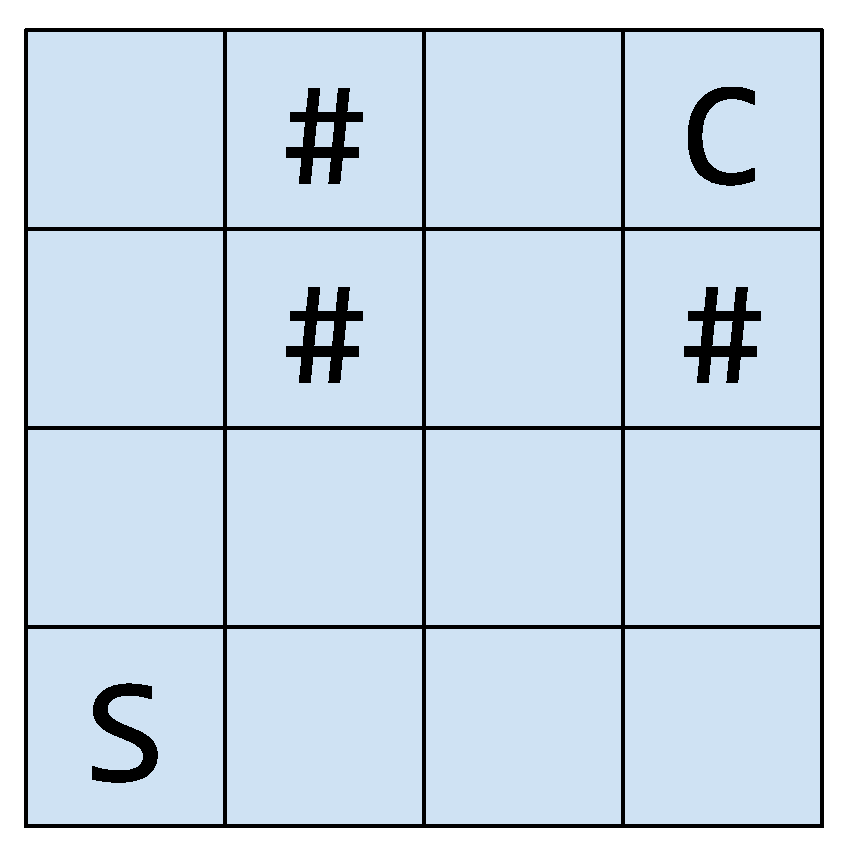
\includegraphics[width=4cm]{portals-example}
	        \end{center}

    }

    \Scoring

    \begin{description}[leftmargin=0pt]
        \item[Apakšuzdevums 1 (? punkti):] $0 \le R \le 10, 0 \le C \le 10$.
        \item[Apakšuzdevums 2 (? punkti):] $0 \le R \le 50, 0 \le C \le 50$.
        \item[Apakšuzdevums 3 (? punkti):] $0 \le R \le 200, 0 \le C \le 200$.
        Katram brīvajam lauciņam balakus ir vismaz viena siena.
				%Every open square has at least one wall adjacent to it.
        \item[Apakšuzdevums 4 (? punkti):] $0 \le R \le 200, 0 \le C \le 200$.
        \item[Apakšuzdevums 5 (? punkti):] $0 \le R \le 1000, 0 \le C \le 1000$.
    \end{description}

    \Constraints

    \begin{description}
        \item[Laika ierobežojums:] ? s.
        \item[Atmiņas ierobežojums:] ? MB.
    \end{description}
\end{document}
